% !TEX program = xelatex
\documentclass[12pt,a4paper]{report}
%\usepackage{polyglossia}
\usepackage{fontspec}
\usepackage{amsmath,amssymb,amsfonts}
\usepackage{graphicx}
\usepackage{float}
\usepackage{subcaption}
\usepackage{xcolor}
\usepackage{listings}
\usepackage{hyperref}
\usepackage{booktabs}
\usepackage{geometry}
\usepackage{titlesec}
\usepackage{algorithm}
\usepackage{algpseudocode}
\usepackage{algorithmicx}

% Set up fonts
\setmainfont[Ligatures=TeX]{Times New Roman}
\setsansfont{Arial}
\setmonofont{Courier New}

% Geometry settings
\geometry{left=2.5cm,right=2.5cm,top=2.5cm,bottom=2.5cm}
\usepackage{ragged2e}

\setlength{\parindent}{0pt}
\setlength{\parskip}{1em}

\emergencystretch=2em
\justifying

\floatname{algorithm}{Αλγόριθμος}
\renewcommand{\listalgorithmname}{Κατάλογος Αλγορίθμων}

\lstset{
	language=Python,
	basicstyle=\ttfamily\footnotesize,
	keywordstyle=\color{blue},
	commentstyle=\color{green!60!black},
	numbers=left,
	numberstyle=\tiny\color{gray},
	stepnumber=1,
	numbersep=5pt,
	backgroundcolor=\color{gray!5},
	showspaces=false,
	showstringspaces=false,
	frame=single,
	tabsize=2,
	breaklines=true,
	captionpos=b
}

\newcommand{\eng}[1]{#1}

\titleformat{\chapter}[display]
{\normalfont\huge\bfseries}{\chaptertitlename\ \thechapter}{20pt}{\Huge}

% Generic named block: \Phase{Title} ... \EndPhase  →  bold header + indent + bold "end"
\algblockdefx[PHASE]{Phase}{EndPhase}[1]{\textbf{#1}}{\textbf{end}}

% Breakable algorithm environment (allows page breaks)
\makeatletter
\newenvironment{breakablealgorithm}
  {%
   \begin{center}
     \refstepcounter{algorithm}%
     \hrule height.8pt depth0pt \kern2pt%
     \renewcommand{\caption}[2][\relax]{%
       {\raggedright\textbf{\ALG@name~\thealgorithm} ##2\par}%
       \ifx\relax##1\relax
         \addcontentsline{loa}{algorithm}{\protect\numberline{\thealgorithm}##2}%
       \else
         \addcontentsline{loa}{algorithm}{\protect\numberline{\thealgorithm}##1}%
       \fi
       \kern2pt\hrule\kern2pt
     }
  }
  {%
     \kern2pt\hrule\relax%
   \end{center}
  }
\makeatother

\begin{document}
	\setlength{\parindent}{0pt}

	% --- Σελίδα τίτλου ---
	\begin{titlepage}
		\centering
		{\LARGE\bfseries ΠΡΟΣΟΜΟΙΩΣΗ ΤΟΥ ΠΡΟΒΛΗΜΑΤΟΣ TAYLOR BEAM \\[.5cm]
		ΜΕ ΤΗ MATERIAL POINT METHOD (MPM)}\\[3cm]

		{\large ΥΠΟΛΟΓΙΣΤΙΚΟ ΘΕΜΑ}\\[1cm]

		{\large ΑΠΟΣΤΟΛΟΠΟΥΛΟΣ ΟΡΦΕΑΣ}\\[0.5cm]
		{\large ΑΜ: 22030}\\[1.5cm]

		{\large ΕΠΙΒΛΕΠΩΝ ΚΑΘΗΓΗΤΗΣ}\\[0.3cm]
		{\large ΙΩΑΝΝΗΣ ΚΑΛΟΓΕΡΗΣ}\\[4.5cm]

		{\large ΤΜΗΜΑ ΜΗΧΑΝΟΛΟΓΩΝ ΜΗΧΑΝΙΚΩΝ}\\
		{\large ΕΘΝΙΚΟ ΜΕΤΣΟΒΙΟ ΠΟΛΥΤΕΧΝΕΙΟ}\\[3cm]

		{\large ΑΘΗΝΑ, ΜΑΪΟΣ 2026}
	\end{titlepage}

	% --- Πίνακας περιεχομένων ---
	\tableofcontents
	\newpage

	% --- Κεφάλαιο 1: Αλγόριθμος ---
	\section{Θεωρητική Εισαγωγή και Αλγόριθμος Υλοποίησης MPM}

	\subsection{Εισαγωγή στην MPM}

	Η Material Point Method (MPM) αναπτύχθηκε αρχικά για την επίλυση προβλημάτων ταχέων μεταβατικών φαινομένων κρούσης (Sulsky et al., 1994) και χρησιμοποιεί ρητό (explicit) επιλύτη, ο οποίος είναι υπολογιστικά πιο αποδοτικός για προβλήματα τέτοιου τύπου σε σύγκριση με έναν πεπλεγμένο (implicit) επιλύτη. Η μέθοδος συνδυάζει τα πλεονεκτήματα της Lagrangian περιγραφής, η οποία επιτρέπει την παρακολούθηση της κατάστασης του υλικού, με εκείνα της Eulerian περιγραφής, η οποία αποφεύγει τα προβλήματα παραμόρφωσης πλέγματος (mesh distortion) κατά την εξέλιξη μεγάλων παραμορφώσεων. Ο συνδυασμός αυτός επιτυγχάνεται με τη χρήση υλικών σημείων (material points / particles), τα οποία λειτουργούν ως φορείς της κατάστασης του υλικού, και ενός σταθερού πλέγματος υποβάθρου (background grid), επί του οποίου επιλύονται οι εξισώσεις κίνησης.

	Από μεθοδολογική άποψη, η MPM μπορεί να θεωρηθεί ως meshfree μέθοδος τύπου Galerkin, συγγενής με τις μεθόδους EFG και RKPM, καθώς επιλύει τις εξισώσεις ορμής στην ασθενή μορφή τους (weak form). Αυτό που τη διαφοροποιεί είναι η απλότητα κατασκευής των συναρτήσεων παρεμβολής (shape functions): πρόκειται για απλά πολυώνυμα (hat functions) ορισμένα επί ενός σταθερού Eulerian πλέγματος, σε αντίθεση με τις υπολογιστικά απαιτητικές και πολύπλοκες συναρτήσεις παρεμβολής άλλων meshfree μεθόδων. Επιπλέον, λόγω του περιοδικού μηδενισμού του πλέγματος σε κάθε χρονικό βήμα, το φαινόμενο παραμόρφωσης πλέγματος δεν εμφανίζεται ποτέ, καθιστώντας την MPM ιδανική για την προσομοίωση προβλημάτων μεγάλων παραμορφώσεων.

	\paragraph{Υπολογιστικός κύκλος.}
	Ένα τυπικό βήμα της ρητής MPM αποτελείται από τέσσερα στάδια, όπως φαίνεται στο Σχήμα~\ref{fig:mpm_overview}:

	\begin{enumerate}
		\item \textbf{P2G (Particle to Grid):} Οι πληροφορίες των σωματιδίων (μάζα, ορμή, δυνάμεις) προβάλλονται στους κόμβους του πλέγματος μέσω των συναρτήσεων παρεμβολής.
		\item \textbf{Grid Updating:} Οι διακριτοποιημένες εξισώσεις ορμής επιλύονται στους κόμβους, ενημερώνοντας τις κομβικές ορμές και ταχύτητες.
		\item \textbf{G2P (Grid to Particles):} Οι ενημερωμένες κομβικές ποσότητες μεταφέρονται πίσω στα σωματίδια προκειμένου να ενημερωθούν θέσεις, ταχύτητες, βαθμίδα παραμόρφωσης (deformation gradient), όγκος και τάσεις.
		\item \textbf{Grid Resetting:} Το πλέγμα μηδενίζεται ώστε να είναι έτοιμο για το επόμενο χρονικό βήμα.
	\end{enumerate}

	Τα βήματα P2G και G2P είναι ανάλογα με αυτά της updated Lagrangian FEM (ULFEM), με τη βασική διαφορά ότι το πλέγμα μηδενίζεται σε κάθε χρονικό βήμα αντί να ακολουθεί το παραμορφούμενο υλικό.

	\begin{figure}[H]
		\centering
		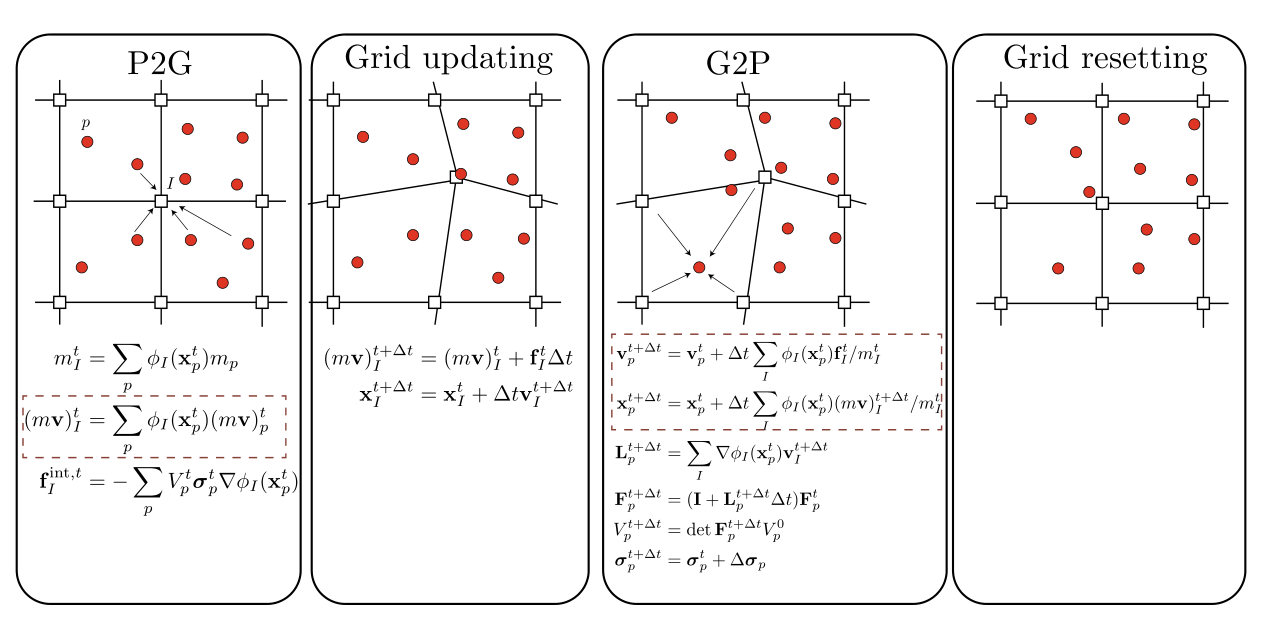
\includegraphics[width=\textwidth]{MPM_overview.png}
		\caption{Τα τέσσερα στάδια του υπολογιστικού κύκλου της MPM: P2G, Grid Updating, G2P και Grid Resetting. Τα βήματα εντός των διακεκομμένων πλαισίων δεν εμφανίζονται στην ULFEM.}
		\label{fig:mpm_overview}
	\end{figure}

	\subsection{Αλγόριθμος Υλοποίησης MPM}

	Ο αλγόριθμος που υλοποιείται είναι η παραλλαγή \emph{MUSL-EP}: συνδυάζει το χρονικό σχήμα ολοκλήρωσης MUSL (Modified Update Stress Last) με ένα ελαστο-πλαστικό (Elasto-Plastic) καταστατικό μοντέλο. Στις ακόλουθες παραγράφους περιγράφονται διαδοχικά (i)~το αριθμητικό πρόβλημα της μικρής κομβικής μάζας και η αντιμετώπισή του μέσω της παραλλαγής MUSL, και (ii)~το καταστατικό μοντέλο που υιοθετείται για την περιγραφή της μηχανικής συμπεριφοράς του υλικού. Στο τέλος της ενότητας παρατίθεται ο πλήρης ψευδοκώδικας του αλγορίθμου.

	\paragraph{Πρόβλημα μικρής μάζας (small mass problem).}
	Κατά τη διάρκεια της προσομοίωσης, κόμβοι που βρίσκονται κοντά στο όριο του υλικού ενδέχεται να αποκτήσουν πολύ μικρή κομβική μάζα $m_I^t$, καθώς ελάχιστα σωματίδια συνεισφέρουν σε αυτούς και μάλιστα με μικρές τιμές της συνάρτησης σχήματος $\phi_I(\mathbf{x}_p^t)$. Η κομβική ταχύτητα υπολογίζεται από τη σχέση:
	\[
		\mathbf{v}_I^t = \frac{(m\mathbf{v})_I^t}{m_I^t} = \frac{\sum_p \phi_I(\mathbf{x}_p^t)\,m_p\,\mathbf{v}_p^t}{\sum_p \phi_I(\mathbf{x}_p^t)\,m_p}
	\]
	Όταν $m_I^t \to 0$, ο λόγος αυτός γίνεται αριθμητικά ασταθής: μικρές διαφορές στον αριθμητή οδηγούν σε ακραίες τιμές της κομβικής ταχύτητας, υπονομεύοντας την ακρίβεια της προσομοίωσης. Το φαινόμενο εικονογραφείται στο Σχήμα~\ref{fig:smallmass}: ο κόμβος~2 βρίσκεται στο όριο του υλικού, επηρεάζεται από ένα μόνο σωματίδιο $p$ με πολύ μικρή τιμή της συνάρτησης σχήματος $N_{2,x}$, με αποτέλεσμα $m_2 \approx 0$ ενώ $f_2 \neq 0$.

	\begin{figure}[H]
		\centering
		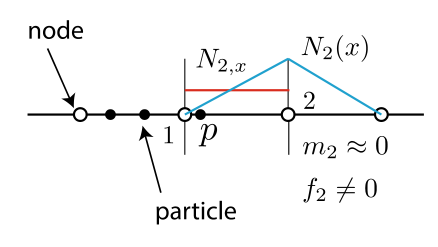
\includegraphics[width=0.55\textwidth]{smallMass.png}
		\caption{Απεικόνιση του προβλήματος μικρής μάζας: ο κόμβος~2 έχει $m_2 \approx 0$ καθώς το σωματίδιο $p$ βρίσκεται σχεδόν εκτός της εμβέλειας της $N_2(x)$, οδηγώντας σε αριθμητική αστάθεια κατά τον υπολογισμό της κομβικής ταχύτητας.}
		\label{fig:smallmass}
	\end{figure}

	Μια συνηθισμένη αντιμετώπιση είναι η επιβολή ενός κατωφλίου (cutoff) στη μάζα: εάν $m_I^t < m_{\mathrm{cut}}$, τότε τίθεται $\mathbf{v}_I^t = \mathbf{0}$. Αν και πρακτικά αποτελεσματική, η προσέγγιση αυτή εισάγει τεχνητή απόσβεση στο σύστημα.

	\paragraph{Αντιμετώπιση μέσω MUSL.}
	Η παραλλαγή Modified Update Stress Last (MUSL) αντιμετωπίζει το πρόβλημα δομικά, χωρίς να προσφεύγει σε τεχνητά κατώφλια. Μετά την ενημέρωση των ταχυτήτων και των θέσεων των σωματιδίων, οι ορμές προβάλλονται εκ νέου στους κόμβους:
	\[
		(m\mathbf{v})_I^{t+\Delta t} = \sum_p \phi_I(\mathbf{x}_p^t)\,(m\mathbf{v})_p^{t+\Delta t}
	\]
	Η κομβική ταχύτητα που χρησιμοποιείται στη συνέχεια κατά το βήμα G2P γίνεται:
	\[
		\mathbf{v}_I^{t+\Delta t} = \frac{(m\mathbf{v})_I^{t+\Delta t}}{m_I^t}
		= \frac{\sum_p \phi_I(\mathbf{x}_p^t)\,(m\mathbf{v})_p^{t+\Delta t}}{\sum_p \phi_I(\mathbf{x}_p^t)\,m_p}
	\]
	Στο δεύτερο κλάσμα, οι συναρτήσεις παρεμβολής $\phi_I$ εμφανίζονται τόσο στον αριθμητή όσο και στον παρονομαστή. Σε έναν κόμβο όπου όλες οι τιμές $\phi_I$ είναι μικρές αλλά ίσες (π.χ. στην ακραία περίπτωση όπου ένα μόνο σωματίδιο συνεισφέρει με $\phi_I = \varepsilon \ll 1$), τα $\varepsilon$ απαλείφονται και η ταχύτητα ισούται με την ταχύτητα του σωματιδίου — παραμένει δηλαδή πεπερασμένη ανεξάρτητα από το πόσο μικρή είναι η κομβική μάζα. Με αυτόν τον τρόπο, το πρόβλημα μικρής μάζας εξαλείφεται χωρίς παράπλευρες απώλειες ακρίβειας.

	Επιπλέον, η MUSL βελτιώνει τη διατήρηση της ορμής σε σύγκριση με τις παραλλαγές USL και USF, γεγονός που την καθιστά προτιμότερη επιλογή για τη συγκεκριμένη εφαρμογή.

	\paragraph{Καταστατικό μοντέλο.}
	Για την περιγραφή της μηχανικής συμπεριφοράς του υλικού υιοθετείται ελαστο-πλαστικό καταστατικό μοντέλο με κριτήριο διαρροής von Mises. Η πλαστική ροή περιγράφεται από το μοντέλο Johnson-Cook (JC), το οποίο αποτυπώνει συνδυαστικά την ισότροπη κράτυνση λόγω πλαστικής παραμόρφωσης, την ευαισθησία στον ρυθμό παραμόρφωσης και τη θερμική χαλάρωση του υλικού:
	\[
		\sigma_f = \underbrace{\bigl[A + B\,(\varepsilon^p)^n\bigr]}_{\text{κράτυνση}}
		\underbrace{\bigl[1 + C\ln\dot{\varepsilon}^*\bigr]}_{\text{ρυθμός}}
		\underbrace{\bigl[1 - (T^*)^m\bigr]}_{\text{θερμοκρασία}}
	\]
	όπου $\dot{\varepsilon}^* = \max(\dot{\varepsilon}/\dot{\varepsilon}_0, 1)$ είναι ο κανονικοποιημένος ρυθμός παραμόρφωσης και $T^* = (T-T_r)/(T_m-T_r)$ η ομόλογη θερμοκρασία. Η πλαστική διόρθωση εφαρμόζεται μέσω του αλγορίθμου radial return (ακτινικής επαναφοράς).

	Για τον υπολογισμό της υδροστατικής πίεσης χρησιμοποιείται η καταστατική εξίσωση Mie-Grüneisen, κατάλληλη για υλικά υπό υψηλές πιέσεις και ταχείες δυναμικές φορτίσεις:
	\[
		\hat{p} = \frac{\rho_0 c_0^2\,\mu\!\left[\eta - \tfrac{\Gamma_0}{2}\mu\right]}{(\eta - S_\alpha\mu)^2} + \Gamma_0\, e, \qquad \eta = \frac{\rho}{\rho_0},\quad \mu = \eta - 1
	\]
	Η εσωτερική ενέργεια $e$ ενημερώνεται αδιαβατικά μέσω του συντελεστή Taylor-Quinney $\chi$, ο οποίος εκφράζει το κλάσμα της πλαστικής εργασίας που μετατρέπεται σε θερμότητα.

	Ο Πίνακας~\ref{tab:material} συνοψίζει τις παραμέτρους του υλικού OFHC Copper που χρησιμοποιήθηκαν στην προσομοίωση.

	\begin{table}[H]
	\centering
	\begin{tabular}{ll|ll|ll}
	\toprule
	\multicolumn{2}{c|}{Παράμετροι υλικού} & \multicolumn{2}{c|}{Παράμετροι Johnson-Cook} & \multicolumn{2}{c}{Παράμετροι EOS} \\
	\midrule
	Πυκνότητα        & $8940\ \mathrm{kg/m^3}$ & $A$ & $65\ \mathrm{MPa}$   & $c_0$        & $3933\ \mathrm{m/s}$ \\
	Ελαστικότητα (Young)      & $115\ \mathrm{GPa}$     & $B$ & $356\ \mathrm{MPa}$  & $S_\alpha$   & $1.5$ \\
	Λόγος Poisson    & $0.31$                  & $C$ & $0.013$              & $\Gamma_0$   & $0$ \\
	                 &                         & $n$ & $0.37$               &              & \\
	\bottomrule
	\end{tabular}
	\caption{Παράμετροι υλικού OFHC Copper για την προσομοίωση Taylor beam.}
	\label{tab:material}
	\end{table}

	Στον ακόλουθο ψευδοκώδικα συγκεντρώνονται όλα τα παραπάνω σε έναν ενιαίο αλγόριθμο: το χρονικό σχήμα MUSL για τη μεταφορά πληροφορίας μεταξύ σωματιδίων και πλέγματος, και η ελαστο-πλαστική καταστατική ενημέρωση για κάθε σωματίδιο εντός του βήματος G2P.

	\begin{breakablealgorithm}
	\caption{Solution Procedure of Explicit MPM with Elasto-Plastic Material (MUSL-EP)}
	\begin{algorithmic}[1]

	\Phase{Initialization}
		\State Set up the Cartesian grid, set time $t = 0$
		\State Set up particle data: $\mathbf{x}_p^0,\ \mathbf{v}_p^0,\ \boldsymbol{\sigma}_p^0,\ \mathbf{F}_p^0,\ V_p^0,\ m_p,\ \rho_p^0$
		\State Set up constitutive data: $\varepsilon_p^{p,0} = 0$,\; ${\boldsymbol{\sigma}'}^{d,0}_p = \mathbf{0}$,\; $e_p^0 = C_v \rho_p^0 (T^0 - T_r)$
	\EndPhase

	\Statex

	\While{$t < t_f$}

		\State \textbf{Reset grid quantities:} $m_I^t = 0,\ (m\mathbf{v})_I^t = \mathbf{0},\ \mathbf{f}_I^{\mathrm{ext},t} = \mathbf{0},\ \mathbf{f}_I^{\mathrm{int},t} = \mathbf{0}$

		\Phase{Mapping from particles to nodes (P2G)}
			\State Compute nodal mass $m_I^t = \sum_p \phi_I(\mathbf{x}_p^t)\, m_p$
			\State Compute nodal momentum $(m\mathbf{v})_I^t = \sum_p \phi_I(\mathbf{x}_p^t)\,(m\mathbf{v})_p^t$
			\State Compute external force $\mathbf{f}_I^{\mathrm{ext},t} = \sum_p \phi_I(\mathbf{x}_p)\, m_p\, \mathbf{b}(\mathbf{x}_p)$
			\State Compute internal force $\mathbf{f}_I^{\mathrm{int},t} = -\sum_p V_p^t\, \boldsymbol{\sigma}_p^t\, \nabla\phi_I(\mathbf{x}_p^t)$
			\State Compute nodal force $\mathbf{f}_I^t = \mathbf{f}_I^{\mathrm{ext},t} + \mathbf{f}_I^{\mathrm{int},t}$
		\EndPhase

		\State \textbf{Update the momenta} $(m\tilde{\mathbf{v}})_I^{t+\Delta t} = (m\mathbf{v})_I^t + \mathbf{f}_I^t\,\Delta t$
		\State \textbf{Fix Dirichlet nodes} $I$: $(m\mathbf{v})_I^t = \mathbf{0}$ and $(m\tilde{\mathbf{v}})_I^{t+\Delta t} = \mathbf{0}$

		\Phase{Update particle velocities and grid velocities (double mapping)}
			\State Get nodal velocities $\tilde{\mathbf{v}}_I^{t+\Delta t} = (m\tilde{\mathbf{v}})_I^{t+\Delta t}/m_I^t$
			\State Update particle positions $\mathbf{x}_p^{t+\Delta t} = \mathbf{x}_p^t + \Delta t\sum_I \phi_I(\mathbf{x}_p^t)\,\tilde{\mathbf{v}}_I^{t+\Delta t}$
			\State Update particle velocities (FLIP/PIC blending, parameter $\alpha$):
			\Statex \hspace{4.5em} $\mathbf{v}_p^{t+\Delta t} = \alpha\!\left(\mathbf{v}_p^t + \textstyle\sum_I \phi_I(\mathbf{x}_p^t)\bigl[\tilde{\mathbf{v}}_I^{t+\Delta t} - \mathbf{v}_I^t\bigr]\right)$
			\Statex \hspace{6em} $+ (1-\alpha)\textstyle\sum_I \phi_I(\mathbf{x}_p^t)\,\tilde{\mathbf{v}}_I^{t+\Delta t}$
			\State Update grid velocities $(m\mathbf{v})_I^{t+\Delta t} = \sum_p \phi_I(\mathbf{x}_p^t)\,(m\mathbf{v})_p^{t+\Delta t}$
			\State Fix Dirichlet nodes $(m\mathbf{v})_I^{t+\Delta t} = \mathbf{0}$
		\EndPhase

		\Phase{Update particles (G2P) and constitutive update}
			\State Get nodal velocities $\mathbf{v}_I^{t+\Delta t} = (m\mathbf{v})_I^{t+\Delta t}/m_I^t$
			\State Compute velocity gradient $\mathbf{L}_p^{t+\Delta t} = \sum_I \nabla\phi_I(\mathbf{x}_p^t)\,\mathbf{v}_I^{t+\Delta t}$
			\State Update deformation gradient $\mathbf{F}_p^{t+\Delta t} = \bigl(\mathbf{I} + \mathbf{L}_p^{t+\Delta t}\,\Delta t\bigr)\mathbf{F}_p^t$
			\State Update volume $V_p^{t+\Delta t} = \det\mathbf{F}_p^{t+\Delta t}\,V_p^0$;\quad update density $\rho_p^{t+\Delta t} = m_p/V_p^{t+\Delta t}$
			\State Strain rate: $\mathbf{D}_p = \tfrac{1}{2}\bigl(\mathbf{L}_p^{t+\Delta t} + {\mathbf{L}_p^{t+\Delta t}}^T\bigr)$
			\State polar decomposition $\mathbf{F}_p^{t+\Delta t} = \mathbf{R}_p\mathbf{U}_p$ extracted via SVD:
			\Statex \hspace{4.5em}  $\mathbf{F}_p = \mathbf{U}_s\,\boldsymbol{\Sigma}\,\mathbf{V}^T \;\Rightarrow\; \mathbf{R}_p = \mathbf{U}_s\mathbf{V}^T$
			\State Un-rotated strain rate and deviatoric part: 
			\Statex \hspace{4.5em} $\mathbf{d}_p = \mathbf{R}_p^T\mathbf{D}_p\mathbf{R}_p$,\; $\mathbf{d}_p^d = \mathbf{d}_p - \tfrac{1}{3}\mathrm{tr}(\mathbf{d}_p)\mathbf{I}$,\; $\dot{\varepsilon}_p = \sqrt{\tfrac{2}{3}\,\mathbf{d}_p^d:\mathbf{d}_p^d}$

			\Phase{Plasticity update (Johnson-Cook)}
				\State Elastic trial deviatoric stress: ${\boldsymbol{\sigma}'}_{\mathrm{trial}}^{d} = {\boldsymbol{\sigma}'}_{p,t}^{d} + 2G\,\Delta t\,\mathbf{d}_p^d$
				\State Trial von Mises stress: $\sigma_{\mathrm{trial}}'^{\,\mathrm{eq}} = \sqrt{\tfrac{3}{2}\,{\boldsymbol{\sigma}'}_{\mathrm{trial}}^{d}:{\boldsymbol{\sigma}'}_{\mathrm{trial}}^{d}}$
				\State JC flow stress with $\dot{\varepsilon}_p^* = \max(\dot{\varepsilon}_p/\dot{\varepsilon}_0,1)$, $T^* = (T-T_r)/(T_m-T_r)$:
					$\sigma_f = \bigl[A+B(\varepsilon_p^{p,t})^n\bigr]\bigl[1+C\ln\dot{\varepsilon}_p^*\bigr]\bigl[1-(T^*)^m\bigr]$
				\If{$\sigma_{\mathrm{trial}}'^{\,\mathrm{eq}} < \sigma_f$} \Comment{elastic step}
					\State ${\boldsymbol{\sigma}'}_{p,t+\Delta t}^{d} = {\boldsymbol{\sigma}'}_{\mathrm{trial}}^{d}$,\quad $\varepsilon_p^{p,t+\Delta t} = \varepsilon_p^{p,t}$,\quad $\Delta\varepsilon_p = 0$
				\Else \Comment{plastic step --- radial return}
					\State $\Delta\varepsilon_p = (\sigma_{\mathrm{trial}}'^{\,\mathrm{eq}} - \sigma_f)/(3G)$,\quad $\varepsilon_p^{p,t+\Delta t} = \varepsilon_p^{p,t} + \Delta\varepsilon_p$
					\State ${\boldsymbol{\sigma}'}_{p,t+\Delta t}^{d} = (\sigma_f/\sigma_{\mathrm{trial}}'^{\,\mathrm{eq}})\,{\boldsymbol{\sigma}'}_{\mathrm{trial}}^{d}$
				\EndIf
			\EndPhase

			\Phase{Pressure update (Mie-Grüneisen EOS)}
				\State Internal energy increment: $\Delta e_p = \det(\mathbf{F}_p)\,\chi\,\sigma_f\,\Delta\varepsilon_p$;\quad $e_p \leftarrow e_p + \Delta e_p$
				\State With $\eta_p = \rho_p^{t+\Delta t}/\rho_p^0$:\quad $-\hat{p}_p = \dfrac{\rho_0 c_0^2(\eta_p-1)\!\left[\eta_p - \frac{\Gamma_0}{2}(\eta_p-1)\right]}{\left[\eta_p - S_\alpha(\eta_p-1)\right]^2} + \Gamma_0\,e_p$
			\EndPhase

			\State Assemble and rotate stress: $\boldsymbol{\sigma'}_{p,t+\Delta t} = {\boldsymbol{\sigma}'}_{p,t+\Delta t}^{d} + \hat{p}_{p,t+\Delta t}\mathbf{I}$;\quad $\boldsymbol{\sigma}_{p,t+\Delta t} = \mathbf{R}_p\boldsymbol{\sigma'}_{p,t+\Delta t}\mathbf{R}_p^T$
			\State Adiabatic temperature update: $T_p^{t+\Delta t} = T_p^t + \chi\,\sigma_f\,\Delta\varepsilon_p\,/\,(\rho_p^{t+\Delta t}C_p)$
		\EndPhase

		\State \textbf{Advance time} $t = t + \Delta t$

	\EndWhile

	\end{algorithmic}
	\end{breakablealgorithm}

	\subsection*{Πίνακας μεταβλητών}

	\begin{table}[H]
	\centering
	\begin{tabular}{ll}
	\toprule
	\textbf{Symbol} & \textbf{Description} \\
	\midrule
	$\phi_I(\mathbf{x}_p^t)$ & Shape function of node $I$ evaluated at particle $p$ \\
	$\mathbf{F}_p$ & Deformation gradient \\
	$\mathbf{R}_p,\ \mathbf{U}_p$ & Rotation and stretch tensors from polar decomposition of $\mathbf{F}_p$ \\
	$\mathbf{D}_p$ & Symmetric strain rate tensor \\
	$\mathbf{d}_p^d$ & Un-rotated deviatoric strain rate \\
	${\boldsymbol{\sigma}'}^d_p$ & Un-rotated deviatoric Cauchy stress \\
	$\varepsilon_p^p$ & Equivalent plastic strain \\
	$\dot{\varepsilon}_p$ & Equivalent strain rate $= \sqrt{\tfrac{2}{3}\mathbf{d}_p^d:\mathbf{d}_p^d}$ \\
	$\dot{\varepsilon}_p^*$ & Normalized strain rate $= \max(\dot{\varepsilon}_p / \dot{\varepsilon}_0,\,1)$ \\
	$T^*$ & Homologous temperature $= (T - T_r)/(T_m - T_r)$ \\
	$A,\,B,\,n,\,C,\,m$ & Johnson-Cook flow stress constants \\
	$G$ & Shear modulus \\
	$K$ & Bulk modulus \\
	$c_0$ & Bulk speed of sound \\
	$\Gamma_0$ & Grüneisen Gamma (reference state) \\
	$S_\alpha$ & Linear Hugoniot slope coefficient \\
	$\chi$ & Taylor-Quinney coefficient \\
	$\alpha$ & FLIP/PIC blending parameter \\
	\bottomrule
	\end{tabular}
	\caption{Variable reference for the MUSL-EP algorithm.}
	\end{table}

	\newpage
	\section{Δομή Κώδικα}
	Η μέθοδος που περιγράφηκε παραπάνω υλοποιήθηκε στην python με την λογική του Object-oriented programming (OOP). Στο directory \texttt{src} υπάρχουν αρχεία οπως: \texttt{mesh2D.py} για την υλοποίηση του πλέγματος υποβάθρου, \texttt{particle.py} για τη διαχείριση των σωματιδίων, \texttt{material.py} για την αποθήκευση των παραμέτρων του υλικού, το \texttt{solver.py} για την υλοποίηση του κύριου αλγόριθμου της MPM κ.α. Το αρχείο \texttt{CopperTaylorImpact.py} περιέχει το κύριο pipeline.

	Ο κώδικας οργανώνεται σε τέσσερα βασικά τμήματα: (1) πλέγμα υποβάθρου (background grid), (2) δομή σωματιδίων (particle data), (3) αρχικοποίηση σωματιδίων (particle generation), (4) αλγόριθμος επίλυσης (solution algorithm) και (5) οπτικοποίηση (visualization). Στις επόμενες ενότητες περιγράφεται αναλυτικά κάθε τμήμα.

	\subsection{Background Grid}

	\begin{figure}[H]
		\centering
		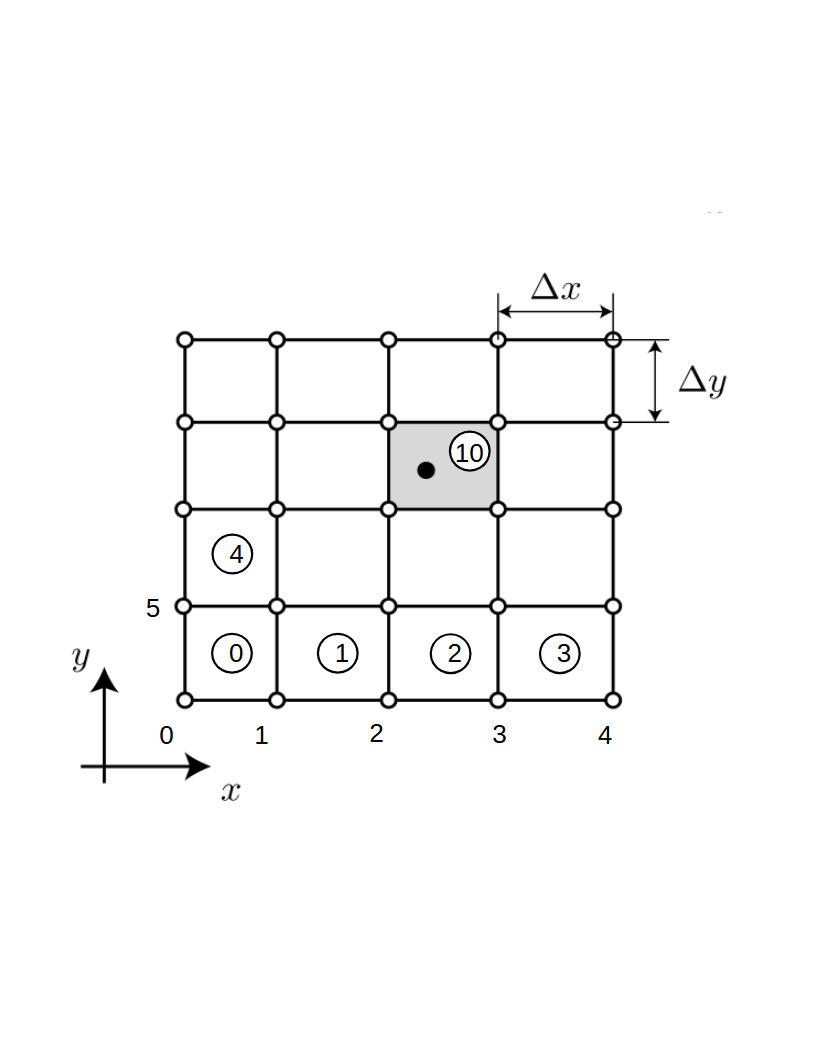
\includegraphics[width=0.55\textwidth]{backroundGrid.png}
		\caption{Δομημένο πλέγμα υποβάθρου με μηδενική αρίθμηση (zero-based) κόμβων και στοιχείων.}
		\label{fig:grid}
	\end{figure}

	Στην MPM χρησιμοποιείται ένα δομημένο καρτεσιανό πλέγμα ως πλέγμα υποβάθρου για την επίλυση των εξισώσεων κίνησης. Η επιλογή ενός ομοιόμορφου τετραγωνικού πλέγματος εξαλείφει την ανάγκη για υπολογιστικά απαιτητικές αναζητήσεις γειτονικών κόμβων κατά την αλληλεπίδραση σωματιδίων-πλέγματος.

	Το πλέγμα ορίζεται από δύο ακέραιους: \texttt{numx} (αριθμός στοιχείων στη διεύθυνση $x$) και \texttt{numy} (αριθμός στοιχείων στη διεύθυνση $y$). Ο συνολικός αριθμός κόμβων είναι $n = (\texttt{numx}+1)(\texttt{numy}+1)$ και ο συνολικός αριθμός στοιχείων $n_{el} = \texttt{numx} \cdot \texttt{numy}$.

	Οι συντεταγμένες των κόμβων αποθηκεύονται σε έναν πίνακα \texttt{nodes} διαστάσεων $n \times 2$, όπου $n$ είναι ο συνολικός αριθμός κόμβων. Κάθε γραμμή αντιστοιχεί σε έναν κόμβο και περιέχει τις συντεταγμένες $(x, y)$:
	\[
	\texttt{nodes} =
	\begin{bmatrix}
		x_0 & y_0 \\
		x_1 & y_1 \\
		\vdots & \vdots \\
		x_{n-1} & y_{n-1}
	\end{bmatrix}
	\]

	Οι κόμβοι των στοιχείων αποθηκεύονται σε έναν πίνακα \texttt{elements} διαστάσεων $n_{el} \times 4$, όπου $n_{el}$ είναι ο αριθμός των στοιχείων. Κάθε γραμμή περιέχει τους δείκτες των τεσσάρων κόμβων του αντίστοιχου στοιχείου (με αντιωρολογιακή σειρά: bottom-left, bottom-right, top-right, top-left):
	\[
	\texttt{elements} =
	\begin{bmatrix}
		n_0^{(0)} & n_1^{(0)} & n_2^{(0)} & n_3^{(0)} \\
		n_0^{(1)} & n_1^{(1)} & n_2^{(1)} & n_3^{(1)} \\
		\vdots    & \vdots    & \vdots    & \vdots    \\
		n_0^{(n_{el}-1)} & n_1^{(n_{el}-1)} & n_2^{(n_{el}-1)} & n_3^{(n_{el}-1)}
	\end{bmatrix}
	\]

	Στην Python η αρίθμηση ξεκινά από το 0 (zero indexing). Οι κόμβοι αριθμούνται γραμμή προς γραμμή ξεκινώντας από κάτω αριστερά, οπότε ο κόμβος με δείκτη $I$ έχει συντεταγμένες:
	\[
	x_I = x_{\min} + (I \bmod n_x)\,\Delta x, \qquad
	y_I = y_{\min} + \left\lfloor \frac{I}{n_x} \right\rfloor \Delta y
	\]
	όπου $n_x = \texttt{numx}+1$ είναι ο αριθμός κόμβων στη διεύθυνση $x$.

	Για ένα δεδομένο στοιχείο με δείκτη $e$, οι τέσσερις κόμβοι του υπολογίζονται ως:
	\begin{align*}
		e_x &= e \bmod \texttt{numx}, \qquad e_y = \left\lfloor e \,/\, \texttt{numx} \right\rfloor \\[4pt]
		n_0 &= e_x + e_y \cdot (\texttt{numx}+1) \\
		n_1 &= n_0 + 1 \\
		n_2 &= n_0 + 1 + (\texttt{numx}+1) \\
		n_3 &= n_0 + (\texttt{numx}+1)
	\end{align*}

	Τα κομβικά μεγέθη (μάζα, ορμή, εσωτερικές και εξωτερικές δυνάμεις) αποθηκεύονται σε NumPy arrays τα οποία μηδενίζονται σε κάθε χρονικό βήμα:
	\[
	\texttt{nmass} =
	\begin{bmatrix} m_0 \\ m_1 \\ \vdots \\ m_{n-1} \end{bmatrix},
	\qquad
	\texttt{nmomentum} =
	\begin{bmatrix}
		(mv)_{x,0} & (mv)_{y,0} \\
		(mv)_{x,1} & (mv)_{y,1} \\
		\vdots & \vdots \\
		(mv)_{x,n-1} & (mv)_{y,n-1}
	\end{bmatrix}
	\]

	Για κάθε σωματίδιο $p$ με θέση $(x_p, y_p)$, ο δείκτης του στοιχείου στο οποίο ανήκει υπολογίζεται ως:
	\begin{equation}\label{eq:p2e}
		e = \left\lfloor \frac{x_p - x_{\min}}{\Delta x} \right\rfloor + \texttt{numx} \cdot \left\lfloor \frac{y_p - y_{\min}}{\Delta y} \right\rfloor
	\end{equation}
	Η αντιστοίχιση των σωματιδίων στα στοιχεία αποθηκεύεται σε μια λίστα \texttt{mpoints} μήκους $n_{el}$, όπου το \texttt{mpoints[e]} επιστρέφει τους δείκτες των σωματιδίων που βρίσκονται εντός του στοιχείου $e$.

	\subsection{Particle Data}

	Τα τυπικά μεγέθη που αποδίδονται σε κάθε σωματίδιο περιλαμβάνουν τη θέση, την ταχύτητα, τη μάζα, τον όγκο, την τάση, την παραμόρφωση, την βαθμίδα παραμόρφωσης (deformation gradient), την ισοδύναμη πλαστική παραμόρφωση, την εσωτερική ενέργεια και τη θερμοκρασία. Τα βαθμωτά μεγέθη (μάζα, όγκος, πυκνότητα, πλαστική παραμόρφωση, ενέργεια, θερμοκρασία) αποθηκεύονται ως μονοδιάστατα NumPy arrays μήκους $n_p$, ενώ τα διανυσματικά και τανυστικά μεγέθη ως δισδιάστατα arrays διαστάσεων $n_p \times k$, όπου $k$ ο αριθμός των ανεξάρτητων συνιστωσών του εκάστοτε μεγέθους.

	\paragraph{Θέση και ταχύτητα.} Αποθηκεύονται ως arrays διαστάσεων $(n_p \times 2)$, με στήλες τις συνιστώσες $x$ και $y$:
	\[
	\texttt{xp} =
	\begin{bmatrix}
		x_0 & y_0 \\
		x_1 & y_1 \\
		\vdots & \vdots \\
		x_{n_p-1} & y_{n_p-1}
	\end{bmatrix}, \qquad
	\texttt{vp} =
	\begin{bmatrix}
		v_{x,0} & v_{y,0} \\
		\vdots & \vdots \\
		v_{x,n_p-1} & v_{y,n_p-1}
	\end{bmatrix}
	\]

	\paragraph{Βαθμίδα παραμόρφωσης (deformation gradient).} Το $\mathbf{F}_p$ είναι τανυστής διαστάσεων $2\times 2$. Αποθηκεύεται ως array $(n_p \times 4)$ με σειρά κατά γραμμές (row-major): $[F_{11},\,F_{12},\,F_{21},\,F_{22}]$. Η αρχικοποίηση γίνεται ως μοναδιαίος τανυστής ($\mathbf{F}_p^0 = \mathbf{I}$), οπότε η πρώτη και η τέταρτη στήλη ισούνται με 1 και οι υπόλοιπες με 0.

	\paragraph{Τάση(cauchy) και αποκλίνουσα(deviatoric) τάση — συμβολισμός Voigt.} Στην περίπτωση επίπεδης παραμόρφωσης (plane strain) στις 2D, ο συμμετρικός τανυστής τάσης Cauchy αποθηκεύεται με τον συμβολισμό Voigt ως array $(n_p \times 3)$ με στήλες $[\sigma_{xx},\, \sigma_{yy},\, \sigma_{xy}]$. Η εκτός επιπέδου συνιστώσα $\sigma_{zz}$ ταυτίζεται με την υδροστατική πίεση $\hat{p}$ και προκύπτει από την εξίσωση κατάστασης. Αντίστοιχα, η αποκλίνουσα τάση ${\boldsymbol{\sigma}'}^d_p$ αποθηκεύεται ως array $(n_p \times 3)$, με την εκτός επιπέδου συνιστώσα να υπολογίζεται από τη συνθήκη μηδενικού ίχνους (traceless condition):
	\[
	s_{zz}^d = -(s_{xx}^d + s_{yy}^d)
	\]
	Αυτή η αναπαράσταση επιτρέπει τον υπολογισμό της ισοδύναμης τάσης von Mises σε επίπεδη παραμόρφωση χωρίς ρητή αποθήκευση της εκτός επιπέδου συνιστώσας:
	\[
	\sigma'^{\,\mathrm{eq}} = \sqrt{\tfrac{3}{2}\,{\boldsymbol{\sigma}'}^d : {\boldsymbol{\sigma}'}^d}
	= \sqrt{\tfrac{3}{2}\bigl(s_{xx}^2 + s_{yy}^2 + s_{zz}^2 + 2s_{xy}^2\bigr)}
	\]

	\paragraph{Βαθμωτά μεγέθη.} Η μάζα $m_p$, ο όγκος $V_p$, ο αρχικός όγκος $V_p^0$, η πυκνότητα $\rho_p$, η ισοδύναμη πλαστική παραμόρφωση $\varepsilon_p^p$, η εσωτερική ενέργεια $e_p$ και η θερμοκρασία $T_p$ αποθηκεύονται ως μονοδιάστατα arrays $(n_p,)$. Ο συνολικός αριθμός σωματιδίων $n_p$ καθορίζεται κατά τη φάση αρχικοποίησης σωματιδίων (particle generation) που περιγράφεται στην επόμενη ενότητα.

	\subsection{Particle Generation}

	Τα σωματίδια τοποθετούνται αρχικά στα σημεία ολοκλήρωσης Gauss-Legendre ενός τετραγωνικού πλέγματος που δημηουργείται για να προσσεγίσει την γεωμετρία του στερεού σώματος. Για ολοκλήρωση βαθμού $n$, κάθε στοιχείο περιέχει $n \times n$ σωματίδια, και ο συνολικός αριθμός σωματιδίων είναι:
	\[
		n_p = n^2 \cdot n_{el:geometry}
	\]

	\paragraph{Τοποθέτηση σωματιδίων.}
	Κάθε στοιχείο απεικονίζεται στο στοιχείο αναφοράς $\hat{\Omega} = [-1,1]\times[-1,1]$ μέσω ενός γραμμικού μετασχηματισμού. Για ομοιόμορφο Cartesian πλέγμα με στοιχείο $e$ που έχει κάτω-αριστερή γωνία $(x_e^0,\, y_e^0)$, οι φυσικές συντεταγμένες των σωματιδίων προκύπτουν από:
	\[
		x_p = x_e^0 + \frac{1+\xi_i}{2}\,\Delta x, \qquad
		y_p = y_e^0 + \frac{1+\eta_j}{2}\,\Delta y
	\]
	όπου $(\xi_i,\, \eta_j)$ είναι τα σημεία Gauss-Legendre στο στοιχείο αναφοράς και $i,j = 0,\ldots,n-1$.

	\paragraph{Αρχικός όγκος σωματιδίου.}
	Ο Ιακωβιανός πίνακας του παραπάνω γραμμικού μετασχηματισμού για ομοιόμορφο πλέγμα είναι διαγώνιος:
	\[
		\mathbf{J}_e =
		\begin{bmatrix} \dfrac{\Delta x}{2} & 0 \\[6pt] 0 & \dfrac{\Delta y}{2} \end{bmatrix}
		\quad\Longrightarrow\quad
		\det(\mathbf{J}_e) = \frac{\Delta x\,\Delta y}{4}
	\]
	Ο αρχικός όγκος κάθε σωματιδίου προκύπτει από τα βάρη ολοκλήρωσης $w_i^\xi,\, w_j^\eta$ και την ορίζουσα του Ιακωβιανού πίνακα:
	\[
		V_p^0 = w_i^\xi\, w_j^\eta\,\det(\mathbf{J}_e) = w_i^\xi\, w_j^\eta\,\frac{\Delta x\,\Delta y}{4}
	\]
	Η ορθότητα της σχέσης επαληθεύεται από τη συνθήκη διατήρησης όγκου:
	\[
		\sum_{i=0}^{n-1}\sum_{j=0}^{n-1} V_p^0 = \Delta x\,\Delta y
	\]
	καθώς $\sum_i w_i^\xi = \sum_j w_j^\eta = 2$ για όλους τους βαθμούς της Gauss-Legendre ολοκλήρωσης.

	\paragraph{Μάζα σωματιδίου.}
	Η μάζα κάθε σωματιδίου υπολογίζεται από τον αρχικό όγκο και την πυκνότητα αναφοράς $\rho_0$:
	\[
		m_p = \rho_0\, V_p^0
	\]
	Η μάζα παραμένει σταθερή καθ' όλη τη διάρκεια της προσομοίωσης, σε συμφωνία με τη Lagrangian φύση των σωματιδίων.

	\paragraph{Αρχικές συνθήκες.}
	Για το πρόβλημα Taylor beam, τα σωματίδια αρχικοποιούνται ως εξής:
	\begin{align*}
		\mathbf{v}_p^0 &= v_0\,\hat{\mathbf{e}}_y & &\text{(αρχική ταχύτητα πρόσκρουσης)} \\
		\boldsymbol{\sigma}_p^0 &= \mathbf{0} & &\text{(αρχικά αφόρτιστη κατάσταση)} \\
		\mathbf{F}_p^0 &= \mathbf{I} & &\text{(απαραμόρφωτη αρχική κατάσταση)} \\
		\varepsilon_p^{p,0} &= 0 & &\text{(μηδενική πλαστική παραμόρφωση)} \\
		T_p^0 &= T_0 & &\text{(ομοιόμορφη αρχική θερμοκρασία)} \\
		e_p^0 &= C_v\,\rho_0\,(T_0 - T_r) & &\text{(αρχική εσωτερική ενέργεια)}
	\end{align*}

	\subsection{Solution Algorithm}

	Το στάδιο επίλυσης υλοποιεί τον αλγόριθμο MUSL-EP που παρουσιάστηκε στην Ενότητα~1. Στις παραγράφους που ακολουθούν περιγράφονται οι κύριες επιλογές που υιοθετήθηκαν κατά την υλοποίηση.

	\paragraph{Συναρτήσεις σχήματος τύπου hat.}
	Ως συναρτήσεις παρεμβολής υιοθετούνται γραμμικές hat (tent) functions, οι οποίες κατασκευάζονται ως γινόμενο δύο μονοδιάστατων τριγωνικών συναρτήσεων:
	\[
		N_I(\mathbf{x}_p) = N_I^x(\xi)\cdot N_I^y(\eta),
		\qquad
		\xi = \frac{x_p - x_I}{\Delta x},\quad \eta = \frac{y_p - y_I}{\Delta y}
	\]
	\[
		N_I^x(\xi) = \begin{cases} 1 - |\xi| & |\xi| < 1 \\ 0 & \text{αλλιώς} \end{cases},
		\qquad
		N_I^y(\eta) = \begin{cases} 1 - |\eta| & |\eta| < 1 \\ 0 & \text{αλλιώς} \end{cases}
	\]
	Λόγω της τοπικής εμβέλειας αυτών των συναρτήσεων, κάθε σωματίδιο αλληλεπιδρά αποκλειστικά με τους τέσσερις κόμβους του στοιχείου εντός του οποίου βρίσκεται. Οι κλίσεις των συναρτήσεων παρεμβολής δίνονται από:
	\[
		\frac{\partial N_I}{\partial x} = -\frac{\mathrm{sign}(\xi)}{\Delta x}\,N_I^y(\eta),
		\qquad
		\frac{\partial N_I}{\partial y} = -\frac{\mathrm{sign}(\eta)}{\Delta y}\,N_I^x(\xi)
	\]

	\paragraph{Υπολογισμός εσωτερικών δυνάμεων (P2G).}
	Οι κομβικές εσωτερικές δυνάμεις υπολογίζονται κατά συνιστώσες, αξιοποιώντας τη μορφή Voigt της τάσης $\boldsymbol{\sigma}_p = [\sigma_{xx},\,\sigma_{yy},\,\sigma_{xy}]$:
	\begin{align*}
		f_{I,x}^{\mathrm{int}} &= -\sum_p V_p \left(\sigma_{xx,p}\,\frac{\partial N_I}{\partial x} + \sigma_{xy,p}\,\frac{\partial N_I}{\partial y}\right) \\
		f_{I,y}^{\mathrm{int}} &= -\sum_p V_p \left(\sigma_{xy,p}\,\frac{\partial N_I}{\partial x} + \sigma_{yy,p}\,\frac{\partial N_I}{\partial y}\right)
	\end{align*}
	Η μοναδική εξωτερική δύναμη που λαμβάνεται υπόψη στη συγκεκριμένη προσομοίωση είναι το βάρος:
	\[
		f_{I,y}^{\mathrm{ext}} = -\sum_p N_I(\mathbf{x}_p)\,m_p\,g
	\]

	\paragraph{Συνοριακές συνθήκες.}
	Για το πρόβλημα Taylor beam εφαρμόζεται μόνο μία συνοριακή συνθήκη: συνθήκη επαφής χωρίς τριβή (frictionless) στο κάτω σύνορο του πεδίου που επιτρέπει την αποκόλιση. Πιο συγκεκριμένα, οι κόμβοι του κάτω συνόρου δεν αποκτούν αρνητική (κατευθυνόμενη προς τα κάτω) ορμή — υλοποιείται ως μονόπλευρος περιορισμός:
	\[
		(m\mathbf{v})_{I,y} \leftarrow \max\!\bigl((m\mathbf{v})_{I,y},\; 0\bigr), \qquad I \in \text{Bottom Nodes}
	\]
	
	\paragraph{Ενημέρωση αντιστοίχισης σωματιδίων-στοιχείων.}
	Καθώς τα σωματίδια κινούνται στον χώρο, ενδέχεται να αλλάξουν στοιχείο. Για τον λόγο αυτό, στο τέλος κάθε χρονικού βήματος υπολογίζεται εκ νέου η αντιστοίχιση σωματιδίων-στοιχείων μέσω της εξίσωσης~\eqref{eq:p2e}, και η λίστα \texttt{mpoints} ανανεώνεται αναλόγως.

	\paragraph{Καταστατική ενημέρωση.}
	Το βήμα G2P και η καταστατική ενημέρωση ακολουθούν πιστά τα βήματα 22–32 του Αλγορίθμου~1 (πλαστικότητα Johnson-Cook, εξίσωση κατάστασης Mie-Grüneisen, αδιαβατική ενημέρωση θερμοκρασίας). Στην παρούσα υλοποίηση δεν περιλαμβάνεται μοντέλο local Damage (Το παράδειγμα 3 point bending περιέχει JC local damage model).

	\subsection{Οπτικοποίηση}

	Σε προκαθορισμένα χρονικά βήματα, τα δεδομένα των σωματιδίων (θέση, ταχύτητα, τάση, αποκλίνουσα τάση, ισοδύναμη πλαστική παραμόρφωση) αποθηκεύονται σε αρχεία μορφής \texttt{.vtp} (VTK Polydata), τα οποία στη συνέχεια οπτικοποιούνται στο ParaView. Κάθε αρχείο αντιστοιχεί σε ένα χρονικό στιγμιότυπο και περιέχει ένα σύνολο από βαθμωτά (scalar) και διανυσματικά (vector) πεδία ανά σωματίδιο.

	Το ParaView επιτρέπει την οπτικοποίηση πεδίων όπως την ισοδύναμη τάση von Mises, την πλαστική παραμόρφωση και την ταχύτητα, καθώς και animations για την παρακολούθηση της εξέλιξης αυτών στον χρόνο. Στο Σχήμα~\ref{fig:paraview} παρουσιάζεται ένα ενδεικτικό στιγμιότυπο της προσομοίωσης Taylor beam.

	\begin{figure}[H]
		\centering
		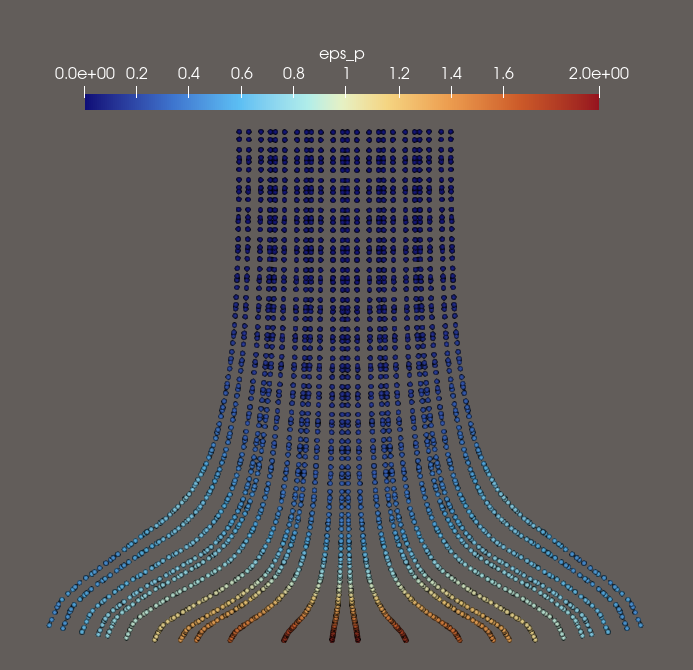
\includegraphics[width=0.75\textwidth]{plasticity_paraview.png}
		\caption{Οπτικοποίηση στο ParaView — ισοδύναμη πλαστική παραμόρφωση $\varepsilon^p$ κατά τη διάρκεια της προσομοίωσης Taylor beam.}
		\label{fig:paraview}
	\end{figure}

	\newpage
	\section{Αποτελέσματα}

	Στον Πίνακα~\ref{tab:geometry} συνοψίζονται η γεωμετρία και οι αρχικές συνθήκες του προβλήματος Taylor beam που χρησιμοποιήθηκαν στις προσομοιώσεις.

	\begin{table}[H]
	\centering
	\begin{tabular}{lll}
	\toprule
	\textbf{Παράμετρος} & \textbf{Σύμβολο} & \textbf{Τιμή} \\
	\midrule
	Διάμετρος ράβδου   & $D$    & $7.6\ \mathrm{mm}$ \\
	Μήκος ράβδου       & $L$    & $25.4\ \mathrm{mm}$ \\
	Αρχική ταχύτητα    & $v_0$  & $190\ \mathrm{m/s}$ \\
	\bottomrule
	\end{tabular}
	\caption{Γεωμετρία και αρχικές συνθήκες του προβλήματος Taylor beam.}
	\label{tab:geometry}
	\end{table}

	\subsection{Έλεγχος Σύγκλισης}

	Για την αξιολόγηση της αριθμητικής σύγκλισης του κώδικα, εκτελέστηκε μια σειρά προσομοιώσεων με διαφορετικό αριθμό σωματιδίων, διατηρώντας σταθερές όλες τις υπόλοιπες παραμέτρους (γεωμετρία, υλικό, χρονικό βήμα, αρχικές συνθήκες). Ως ποσότητες αναφοράς για τη σύγκλιση επιλέχθηκαν δύο γεωμετρικά μεγέθη που μετρούνται και πειραματικά στο κλασικό πείραμα Taylor beam:

	\begin{itemize}
		\item $\Delta L / L$: σχετική αξονική συμπίεση (shortening) της ράβδου μετά την πρόσκρουση
		\item $\Delta D / D$: σχετική ακτινική διαστολή (radial expansion) της βάσης της ράβδου
	\end{itemize}

	Το Σχήμα~\ref{fig:convergence} παρουσιάζει την εξάρτηση των δύο αυτών ποσοτήτων από τον αριθμό των σωματιδίων.

	\begin{figure}[H]
		\centering
		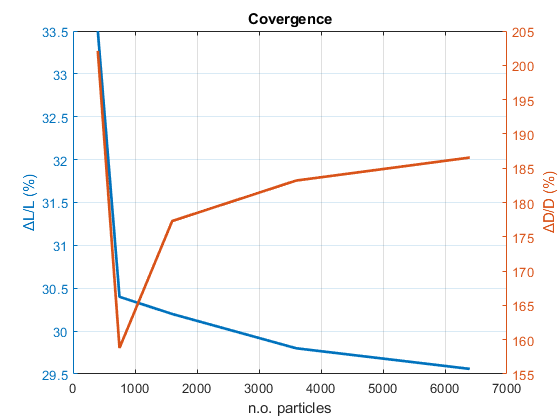
\includegraphics[width=0.75\textwidth]{data_analysis/convergence.png}
		\caption{Έλεγχος σύγκλισης: σχετική αξονική συμπίεση $\Delta L/L$ (μπλε, αριστερός άξονας) και σχετική ακτινική διαστολή $\Delta D/D$ (πορτοκαλί, δεξιός άξονας) συναρτήσει του αριθμού σωματιδίων.}
		\label{fig:convergence}
	\end{figure}

	Παρατηρείται ότι αμφότερες οι ποσότητες παρουσιάζουν έντονη μεταβολή για χαμηλό αριθμό σωματιδίων ($n_p \lesssim 750$), ενώ σταθεροποιούνται σταδιακά για $n_p \gtrsim 2000$. Συγκεκριμένα, το $\Delta L/L$ συγκλίνει προς την τιμή $\approx 29.6\%$ και το $\Delta D/D$ προς $\approx 185\%$. Η συμπεριφορά αυτή επιβεβαιώνει ότι το αποτέλεσμα δεν εξαρτάται από τον αριθμό των σωματιδίων πέρα από ένα ορισμένο επίπεδο διακριτοποίησης, γεγονός που υποδηλώνει ότι έχει επιτευχθεί αριθμητική σύγκλιση.

	\subsection{Σύγκριση με ANSYS Explicit}

	Για την επαλήθευση των αποτελεσμάτων του MPM κώδικα πραγματοποιήθηκε σύγκριση με αντίστοιχη προσομοίωση στο ANSYS Explicit. Το ίδιο πρόβλημα Taylor beam μοντελοποιήθηκε με τη Μέθοδο των Πεπερασμένων Στοιχείων (FEM), χρησιμοποιώντας τετράπλευρα στοιχεία (quad elements) σε επίπεδη παραμόρφωση και το ίδιο καταστατικό μοντέλο (πλαστικότητα Johnson-Cook, εξίσωση κατάστασης Mie-Grüneisen). Στο Σχήμα~\ref{fig:comparison} παρουσιάζονται στιγμιότυπα από τις δύο προσομοιώσεις.

	\begin{figure}[H]
		\centering
		\begin{subfigure}{0.48\textwidth}
			\centering
			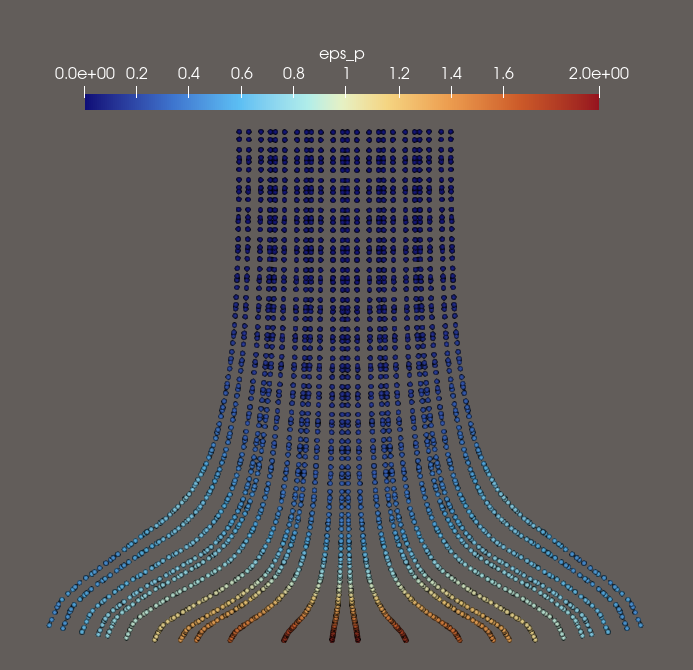
\includegraphics[width=\textwidth]{plasticity_paraview.png}
			\caption{MPM (ParaView)}
			\label{fig:mpm_snap}
		\end{subfigure}
		\hfill
		\begin{subfigure}{0.48\textwidth}
			\centering
			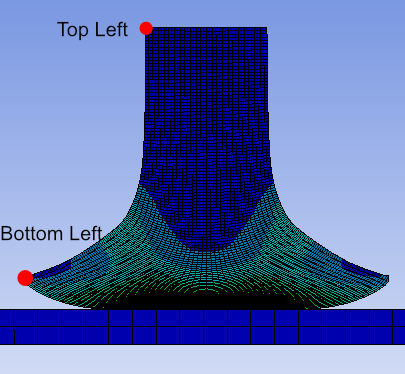
\includegraphics[width=\textwidth]{ansys_bar.png}
			\caption{FEM — ANSYS Explicit}
			\label{fig:ansys_snap}
		\end{subfigure}
		\caption{Σύγκριση στιγμιότυπων MPM και ANSYS Explicit. Χρωματισμός βάσει ισοδύναμης πλαστικής παραμόρφωσης $\varepsilon^p$.}
		\label{fig:comparison}
	\end{figure}

	Στο Σχήμα~\ref{fig:disp_compare} παρουσιάζεται η χρονική απόκριση της μετατόπισης σε δύο χαρακτηριστικά σημεία της ράβδου — κάτω-αριστερά (βάση, σημείο επαφής) και πάνω-αριστερά (ελεύθερο άκρο) — για τις δύο μεθόδους. Παρατηρείται ότι οι καμπύλες των MPM και ANSYS Explicit ακολουθούν παρόμοια μορφή: τόσο οι μέγιστες τιμές όσο και η χρονική εξέλιξη της μετατόπισης συμφωνούν ικανοποιητικά, παρά τις μικρές αποκλίσεις που οφείλονται στη διαφορετική διακριτοποίηση και στη διαφορετική φύση των δύο μεθόδων (meshfree MPM έναντι FEM).

	\begin{figure}[H]
		\centering
		\begin{subfigure}{0.48\textwidth}
			\centering
			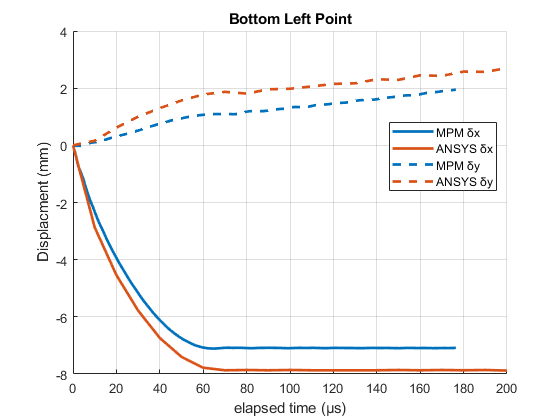
\includegraphics[width=\textwidth]{data_analysis/bottom_left_compare.png}
			\caption{Μετατόπιση κάτω-αριστερά κόμβου}
			\label{fig:disp_bottom}
		\end{subfigure}
		\hfill
		\begin{subfigure}{0.48\textwidth}
			\centering
			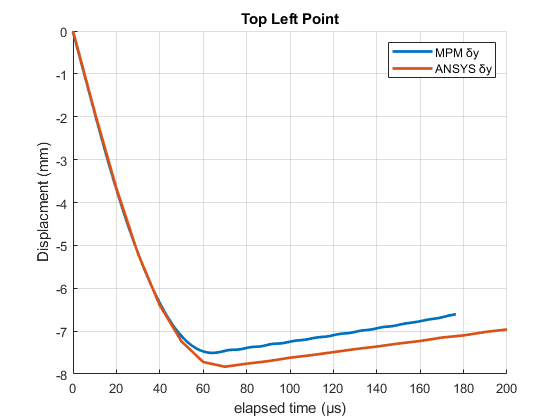
\includegraphics[width=\textwidth]{data_analysis/top_left_compare.png}
			\caption{Μετατόπιση πάνω-αριστερά κόμβου}
			\label{fig:disp_top}
		\end{subfigure}
		\caption{Σύγκριση χρονικής απόκρισης μετατόπισης MPM και ANSYS Explicit στα κάτω και πάνω αριστερά άκρα. Οι δύο μέθοδοι παρουσιάζουν παρόμοια συμπεριφορά με μικρές αποκλίσεις.}
		\label{fig:disp_compare}
	\end{figure}

	Στο Σχήμα~\ref{fig:bar_compare} παρουσιάζεται η ποσοτική σύγκριση των δύο βασικών γεωμετρικών μεγεθών — της σχετικής αξονικής συμπίεσης $\Delta L/L$ και της σχετικής ακτινικής διαστολής $\Delta D/D$ — μεταξύ MPM και ANSYS Explicit. Οι ποσότητες συμφωνούν ικανοποιητικά, επιβεβαιώνοντας την εγκυρότητα του MPM κώδικα, παρά τις μικρές αποκλίσεις που είναι αναμενόμενες λόγω της διαφορετικής φύσης των δύο μεθόδων.

	\begin{figure}[H]
		\centering
		\begin{subfigure}{0.48\textwidth}
			\centering
			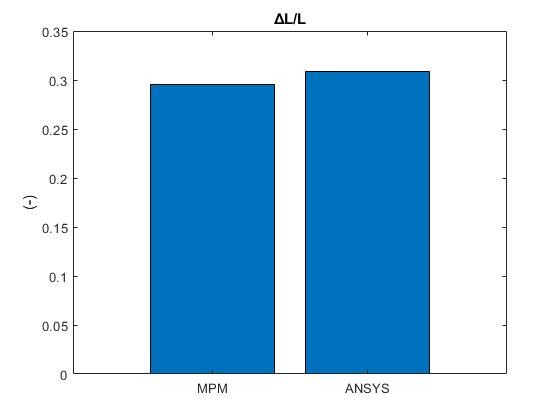
\includegraphics[width=\textwidth]{data_analysis/compareDL_L.png}
			\caption{Σχετική αξονική βράχυνση $\Delta L/L$}
			\label{fig:bar_dl}
		\end{subfigure}
		\hfill
		\begin{subfigure}{0.48\textwidth}
			\centering
			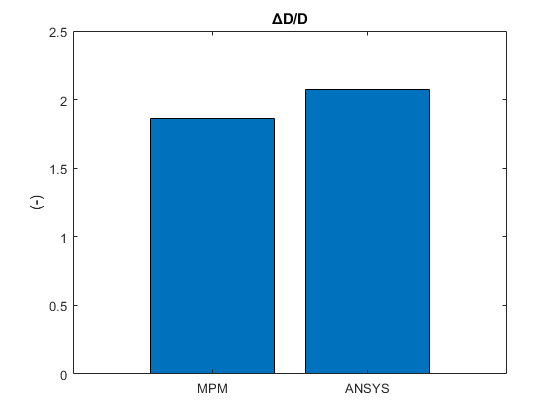
\includegraphics[width=\textwidth]{data_analysis/compareDD_D.png}
			\caption{Σχετική ακτινική διαστολή $\Delta D/D$}
			\label{fig:bar_dd}
		\end{subfigure}
		\caption{Σύγκριση γεωμετρικών αποτελεσμάτων MPM και ANSYS Explicit. Οι τιμές των δύο μεθόδων συμφωνούν ικανοποιητικά, με μικρές αποκλίσεις που οφείλονται στη διαφορετική διακριτοποίηση και φύση των μεθόδων.}
		\label{fig:bar_compare}
	\end{figure}

\end{document}
